\documentclass[12pt]{article}
\usepackage[margin=1.2in]{geometry}
\usepackage{amsmath}
\usepackage{ctex}
\usepackage{siunitx}
\usepackage{graphicx}
\usepackage{subcaption}
\usepackage{gensymb} 
\usepackage{xcolor}
\usepackage{soul} 
\usepackage{tcolorbox} 
\usepackage{float} 
\newtcolorbox[auto counter, number within=section]{highlightedsection}[2][]{colframe=cyan!80!black, colback=cyan!30, coltitle=black, sharp corners, fonttitle=\bfseries, title=#2,#1}

\title{实验二\,\,七段数码管动态显示电路设计报告}
\author{姓名：怀迪\,\, 学号：PB23061112 \\ }
\date{}
 
\begin{document}
\maketitle

% 使用 tcolorbox 使标题带有荧光笔效果
\begin{highlightedsection}{}
    一、实验内容简述
\end{highlightedsection}
本次实验大体上是要求我们编写Verilog代码实现一个七段数码管动态显示电路设计，并在
Quartus软件中进行仿真和FPGA验证。

需要实现的具体功能:根据输入的位选信号（3位）选择需要改变输出内容的数码管；
然后输入数据信号（4位），来控制输出的8个阳极共通的数码管（每一个阳极对应一整个七段数码管）
的7个阴极（对应每一个数码管显示的数字）；
最后发送使能信号，改变数码管上的数字显示。



\begin{highlightedsection}{}
    二、设计分析
\end{highlightedsection}
\subsection*{1.实验题目分析}
首先我们需要确认输入输出信号一共需要8位：3位位选信号+4位数据信号
+1位使能信号+1个clk信号。

3位位选信号需要用来选择8个数码管中的一个进行改变数值，4位数据信号
用来给不同的数码管进行赋值，1位使能信号用来控制数码管的显示改变与否，clk信号用来循环显示
数码管。

而输出需要控制8个数码管的8个阴极信号+控制数码管LED灯显示的8个信号，一共十六位。

明确了输入信号输出信号的数量我们就需要思考如何进行功能实现：
首先我们需要一个计数器来对clk信号进行分频（分频前clk为50Mhz，过大），
然后我们需要根据位选信号选择寄存器来存储数码管的数值，
之后我们需要一个循环计数器来循环选择数码管显示其对应寄存器存储的数值，
循环显示的频率为分频后的信号频率，
最后根据寄存器的数值来解码成LED灯的阴极信号以实现数字显示。

\subsection*{2.编程思路}
我把代码分成了三个模块:实现具体功能的顶层模块，分频模块和解码信号模块。
\subsubsection*{2.1 顶层模块}
顶层模块主要实现对输入信号的处理和对其他两个模块的调用。
首先调用分频模块对clk信号进行分频，得到一个较低频率的时钟信号clk\_divided。

然后根据想要改变数值的数码管选择寄存器进行赋值，
使用一个case语句根据3位位选信号选择对应的寄存器进行赋值操作。

接着使用一个循环计数器根据分频后的时钟信号循环选择数码管进行显示，
使用一个case语句根据循环计数器的值选择对应的数码管进行显示。

最后调用解码模块将寄存器的数值解码成对应的阴极信号。
\subsubsection*{2.2 分频模块}
分频模块主要实现对输入的clk信号进行分频操作。

首先输入未分频的时钟信号，使用一个计数器对输入的clk信号进行计数，当计数器达到设定的分频值时，
翻转输出的分频信号，并将计数器清零。

此时得到的输出信号为分频后的时钟信号clk\_divided。
\subsubsection*{2.3 解码模块}
解码模块主要实现将4位二进制数值解码成对应的七段数码管阴极信号。

首先输入4位二进制数值，使用一个case语句根据输入的数值选择对应的七段数码管阴极信号。

输出对应的七段数码管阴极信号以实现数字显示。
\begin{highlightedsection}{}
    三、VHDL源代码
\end{highlightedsection}
本代码实现了分频时钟作为输入，选择相应寄存器并手动输入数据实现更改数码管显示内容
的功能，同时实现循环选择数码管进行动态显示的功能。其中，每次更改数码管显示内容的时候，
需要将使能信号拉低，完成更改后再拉高。我还添加了复位功能，当复位信号拉低时，
所有寄存器置位，数码管显示1-8。
\begin{figure}[ht]
    \centering
    % 第一张图，宽度 0.45 页宽
    
\includegraphics[width=0.41\textwidth]{代码1.png}
    \quad  % 两图之间添加固定间隙（比 \hfill 间距小）
    % 第二张图
    
\includegraphics[width=0.54\textwidth]{代码2.png}
    \caption{设计代码1-92行图片}
\end{figure}

\begin{figure}[ht]
    \centering
    % 第一张图，宽度 0.45 页宽
    
\includegraphics[width=0.42\textwidth]{代码3.png}
    \quad  % 两图之间添加固定间隙（比 \hfill 间距小）
    % 第二张图
    
\includegraphics[width=0.42\textwidth]{代码4.png}
    \caption{设计代码93-149行图片}
\end{figure}

\newpage
\begin{highlightedsection}{}
    四、仿真结果记录
\end{highlightedsection}
\begin{figure}[H]  % H 表示固定图片位置
    \centering
    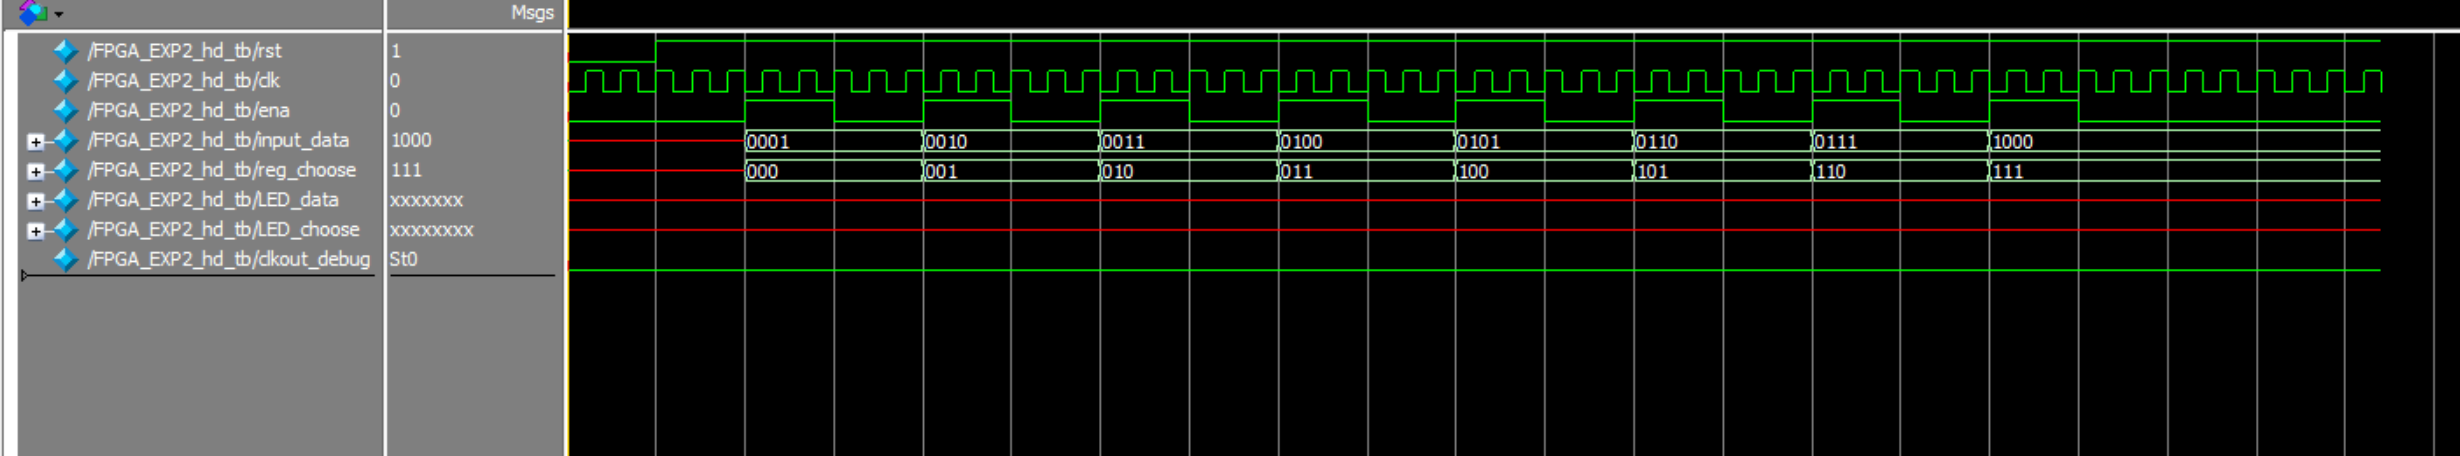
\includegraphics[width=\textwidth]{仿真.png}  % 图片的最大宽度为文本宽度
\end{figure}
仿真结果如上图所示，首先复位信号拉低，所有寄存器置位，数码管显示1-8；

然后复位信号拉高，顺序选择数码管更改数值，分别将数码管1-8更改为1、2、3、4、5、6、7、8，
每次更改数值时使能信号拉低，完成更改后使能信号拉高。

可能是软件原因，仿真波形图中数码管显示的内容没有体现出来，
但实际上代码逻辑是正确的，FPGA验证结果也符合预期。后续有待进一步排查。
\begin{highlightedsection}{}
    五、FPGA验证结果记录
\end{highlightedsection}
我选择DIP0-2作为位选信号输入，DIP3-6作为数据信号输入，
DIP7作为使能信号输入，DIP8作为复位信号输入，
FPGA板载时钟作为clk信号输入。

代码烧写进去后，我通过拨动DIP开关来改变数码管的显示内容，
验证结果与预期一致，数码管能够正确显示对应的数字。

初始复位结果如下图所示，数码管显示数字1-8：
\begin{figure}[H]  % H 表示固定图片位置
    \centering
    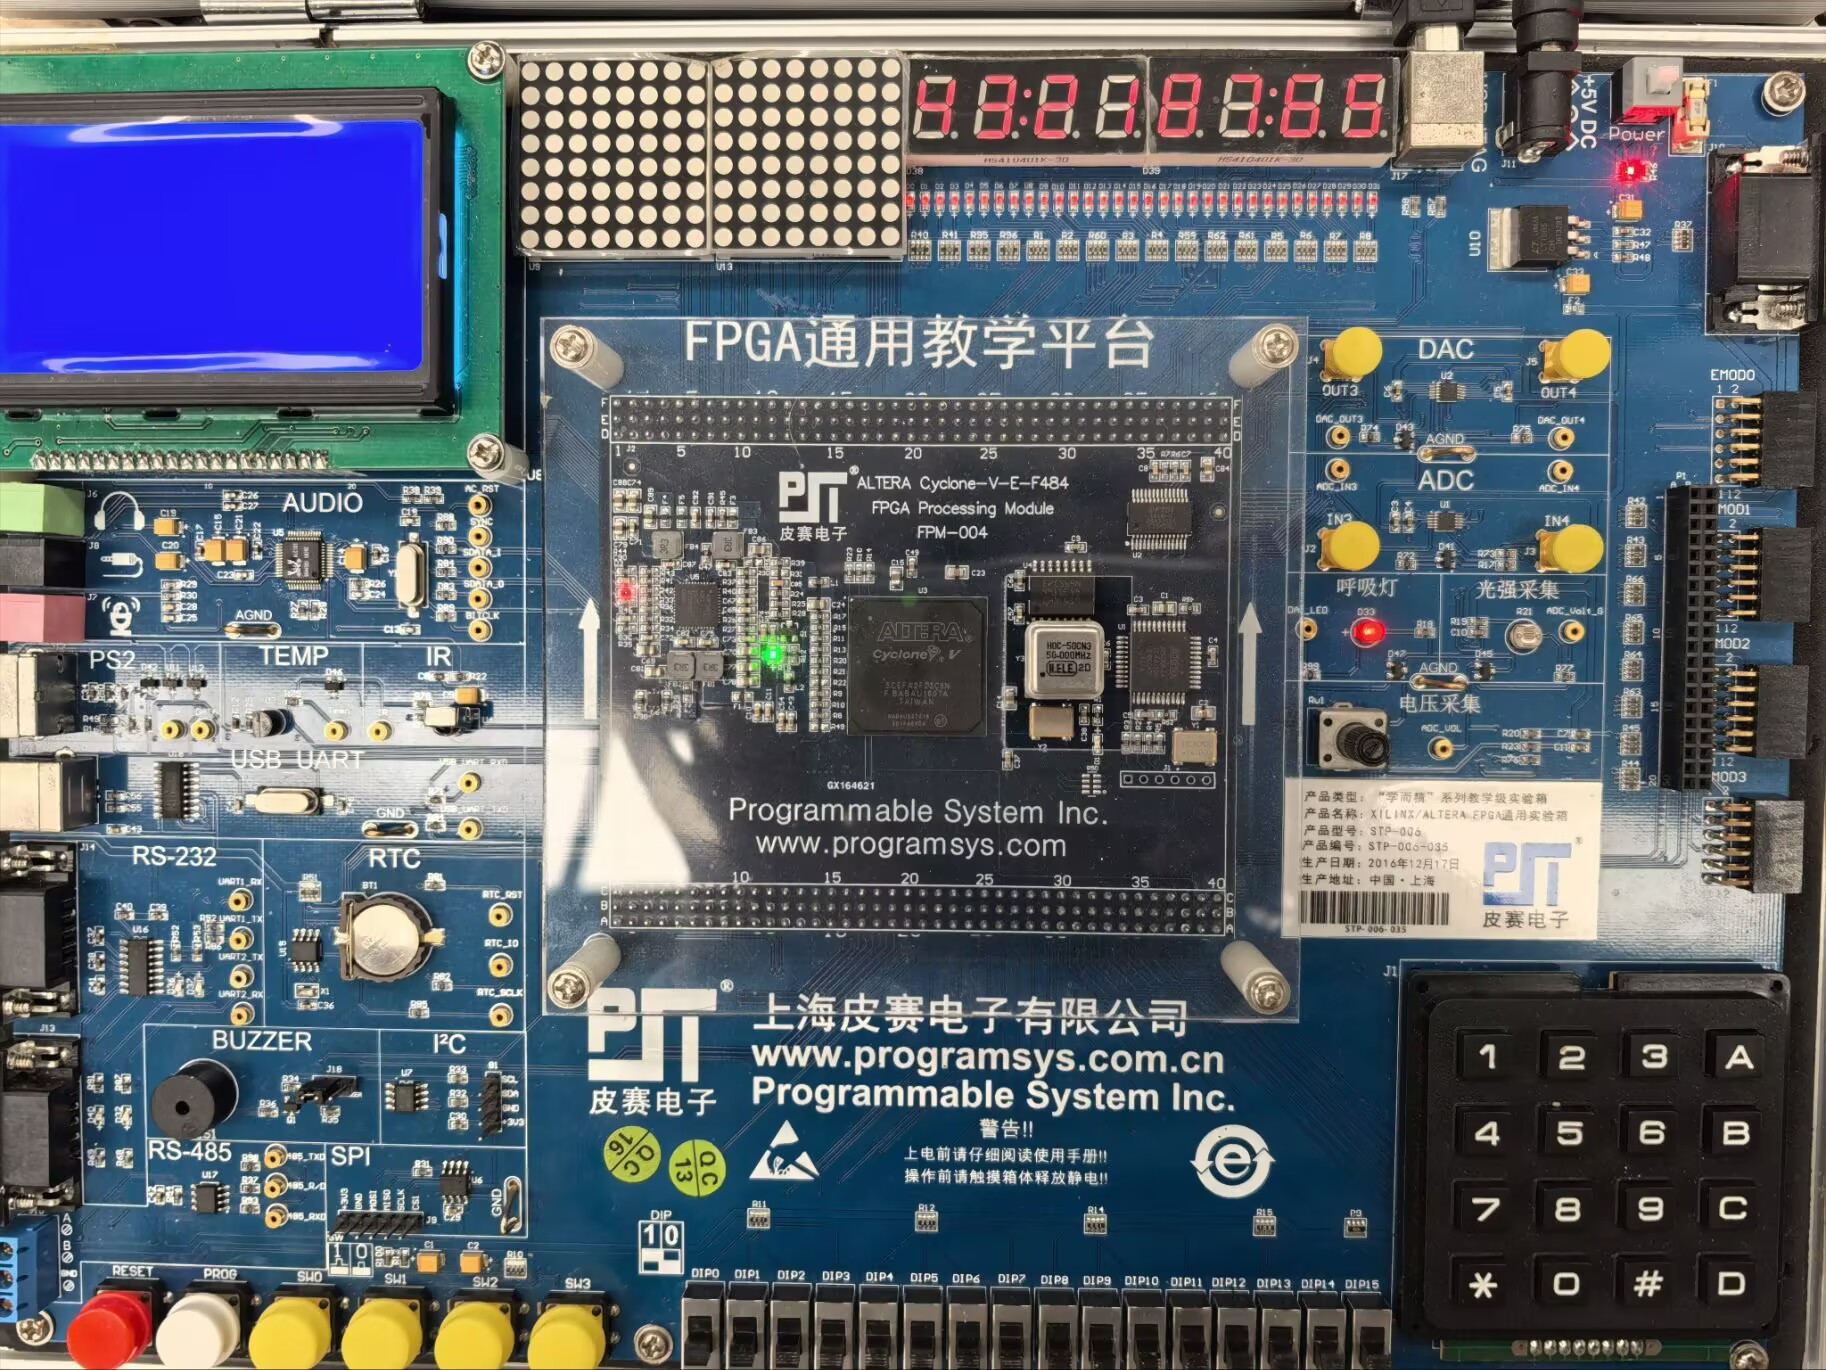
\includegraphics[width=0.9\textwidth]{数码管1.jpg}  % 图片的最大宽度为文本宽度
\end{figure}

随后我更改数码管1显示内容为3，结果如下图所示，数码管能够正确显示对应的数字：
\begin{figure}[H]  % H 表示固定图片位置
    \centering
    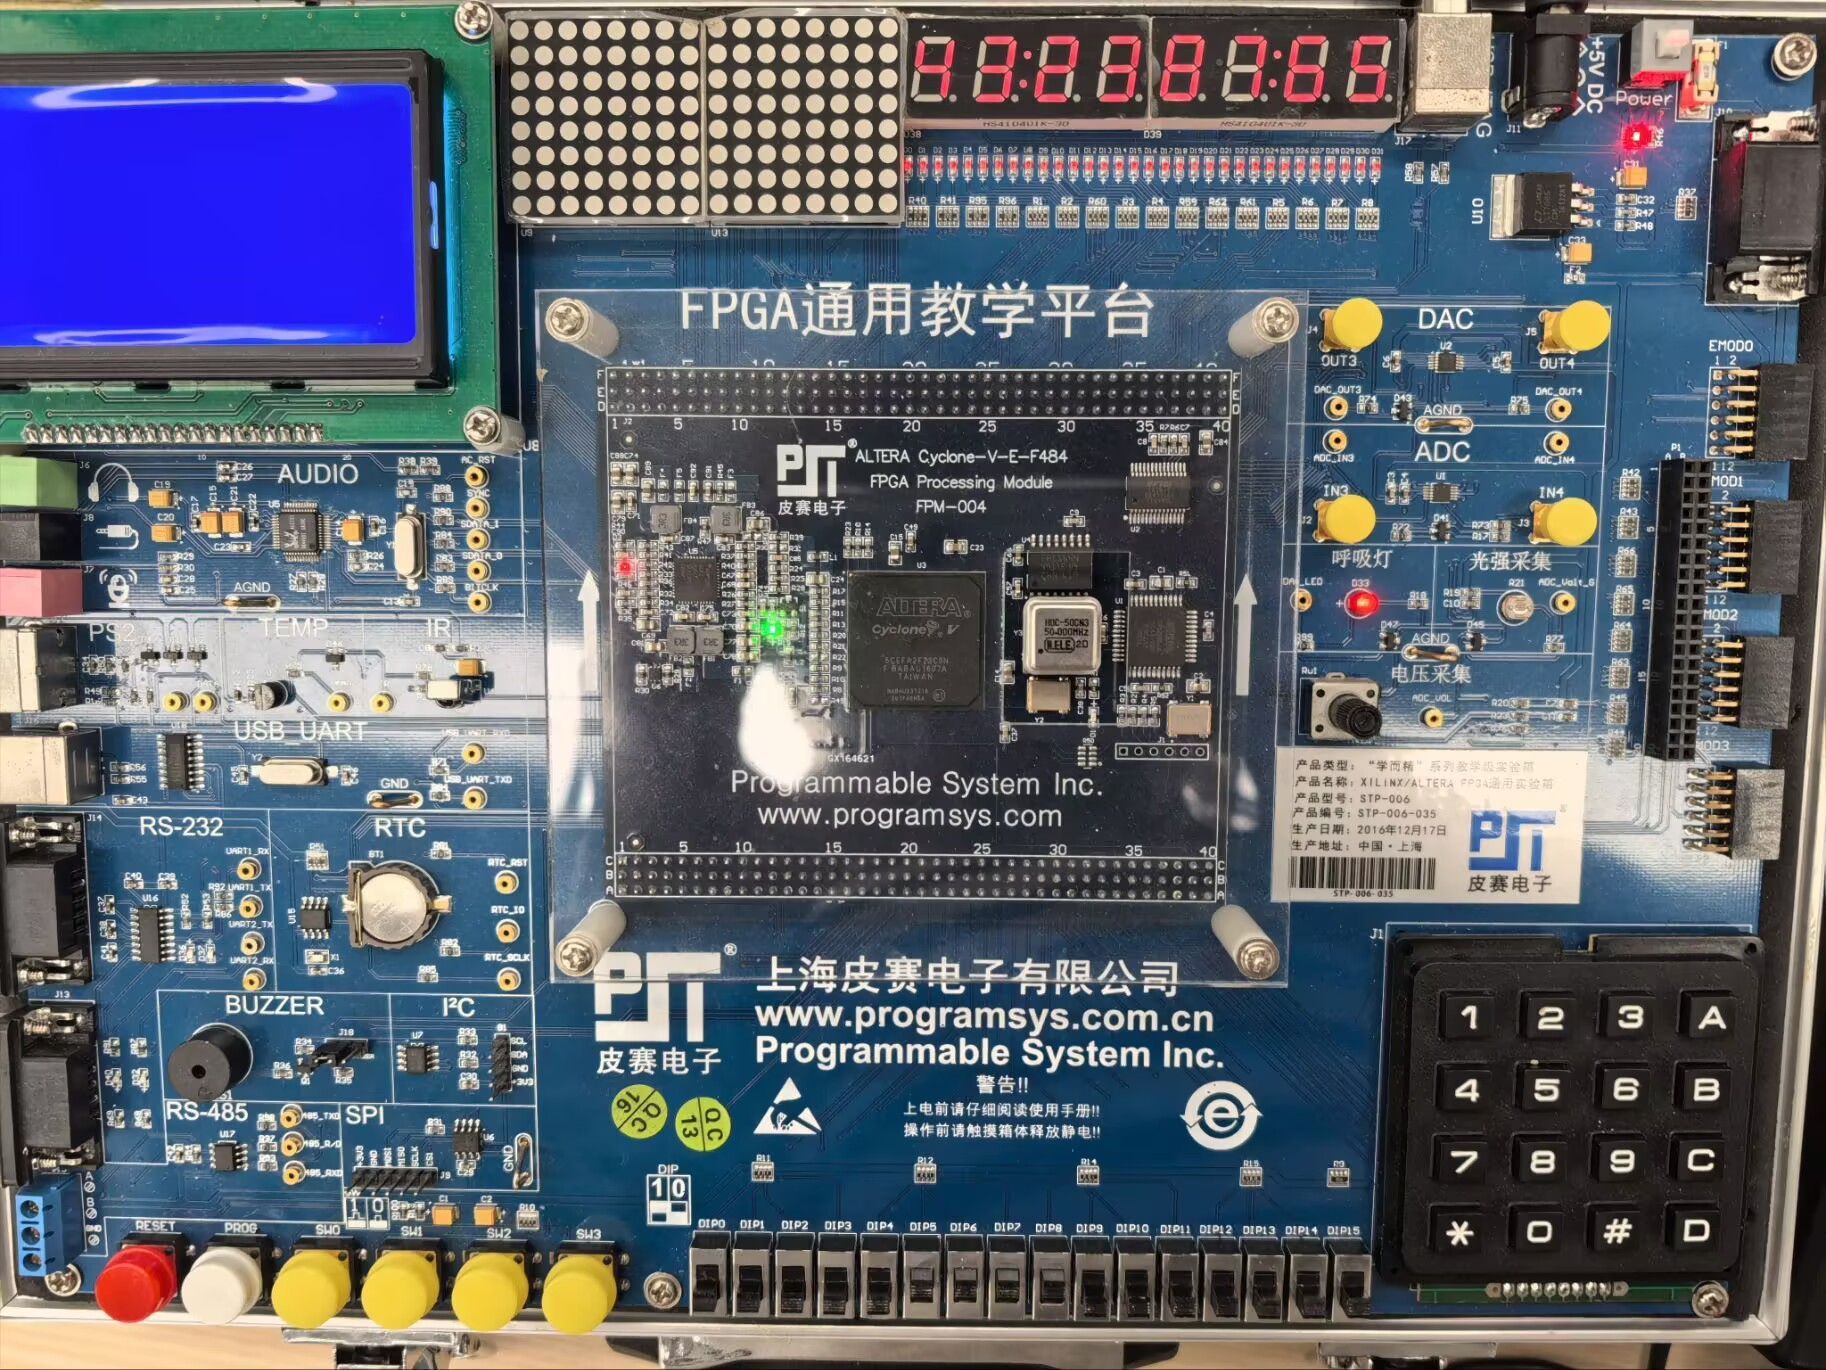
\includegraphics[width=0.9\textwidth]{数码管2.jpg}  % 图片的最大宽度为文本宽度
\end{figure}
随后更改其余数码管的数字，结果均符合预期，验证成功。

此外，每次改变后拉低reset信号，数码管均能正确复位显示1-8，验证成功。

\begin{highlightedsection}{}
    六、实验总结
\end{highlightedsection}
本次实验相对于实验一来说难度有所提升，需要我们综合运用之前所学的知识来
实现一个较为复杂的电路设计。

刚开始设计电路的时候，编译过后代码一直报错，后面我结合ai排查了一下，发现是
wire类型的数据不能在always模块中进行赋值操作，修改为reg类型后问题解决。

后面在实验过程中，我发现赋值操作基本能正常运行，但是一使用复位功能，数码管
就只会显示其中一位数字，并且是随机显示其中一个数码管，后面经过排查发现是我在分频
模块中加入了复位信号的判断，导致我复位时分频模块的输出信号一直是同一个电平
，无法正确输出分频后的时钟信号，修改后问题解决。

本次实验我收获颇多，不仅加深了我对Verilog编程的理解，
还提升了我解决实际问题的能力，更让我意识到了模块分开书写的重要性。
\end{document}